% ============================================
%  Article Class (This is a LaTeX2e document)  
% ============================================
\documentclass[12pt]{scrartcl}
\usepackage[english]{babel}
\usepackage{enumitem}
\usepackage[round]{natbib}
\usepackage{color}

\newcommand\reft[3][]{#2~\ref{#3}#1}
\newcommand\refp[3][]{(#2~\ref{#3}#1)}
\newcommand\refsect[1]{\reft{Section}{#1}}
\newcommand\refsecp[1]{\refp{Sec.}{#1}}
\newcommand\reftabt[1]{\reft{Table}{#1}}
\newcommand\reftabp[1]{\refp{Tab.}{#1}}

% ============
%  Algorithms
% ============
\usepackage{algorithm2e}
\SetKwProg{Fn}{Function}{}{}
\newcommand\refalgt[1]{\reft{Algorithm}{#1}}
\newcommand\refalgp[1]{\refp{Alg.}{#1}}

% ======
%  Math
% ======
\usepackage{amsmath}
\usepackage{amsthm}
\newtheorem{thm}{Theorem}[section]
\newtheorem{cor}[thm]{Corollary}
\newtheorem{lem}[thm]{Lemma}
\newtheorem{prop}[thm]{Proposition}
\newtheorem{property}[thm]{Property}
\theoremstyle{definition}
\newtheorem{defn}[thm]{Definition}
\newtheorem{assum}[thm]{Assumption}
\theoremstyle{remark}
\newtheorem{rem}[thm]{Remark}
\numberwithin{equation}{section}
\usepackage{amssymb}
\newcommand{\prob}[1]{\mathbb{P}\left(#1\right)}

% ====================
%  Chemical reactions
% ====================
\usepackage[version=3]{mhchem}
\newcommand{\reactionRev}[4]{#1 \ce{<=>[#3][#4]} #2}
\newcommand{\reactionIrr}[4]{#1 \ce{->[#3][#4]} #2}

% ============================
%  Figures and relative paths
% ============================
\usepackage{graphicx}
\graphicspath{{figures/}}
\usepackage{import}
\makeatletter
  \def\relativepath{\import@path}
\makeatother
\newcommand\reffigt[2][]{\reft[#1]{Figure}{#2}}
\newcommand\reffigp[2][]{\refp[#1]{Fig.}{#2}}

% ==========
%  Document
% ==========
\begin{document}

\title{{CATI MIAGO}: comparing algorithms for Gillespie based simulations}%
\author{M.~Dinh, S.~Fischer, A.~Goelzer}%
\date{\today}%

\maketitle

\newpage

\tableofcontents

\newpage

\section{Introduction}

Gillespie's algorithm was designed to simulate chemical reaction networks, even in conditions where there are only a few molecules. In this section we briefly present how it was conceived and implemented.

\subsection{Principles underlying Gillespie's algorithm}

We suppose we are given a set of chemical reactions that we can write, in general as
\[
\reactionRev{a_1A_1 + a_2A_2 + ... + a_rA_r}{b_1B_1+..+b_pB_p}{k_1}{k_{-1}}
\]
the simplest reaction being a complexation reaction of the form
\[
\reactionRev{A + B}{C}{k_1}{k_{-1}}
\]

\begin {assum}[Well-mixed medium] 
  The first important hypothesis is that the molecules of every chemical species are distributed uniformly across space at all times. Then the probability that a molecule of species $A$ encounters a molecule of species $B$ is proportional to $n_An_B$ where $n_A$ is the number of molecules of species A and $n_B$ the number of molecules of species $B$. Note that the probability that a molecule of species $A$ encounters another molecule of species $A$ is proportional to $n_A(n_A-1)$.
\end {assum}

\begin {assum}[Low-order reactions] 
  The second hypothesis is that reactions represent low-order phenomena, \textit{i.e.} they result uniquely of the concomitant encounter of all species involved (as opposed to a sequence of events implying one or the other species).
\end {assum}

\begin {defn}[Propensity] 
  The propensity of a reaction is the rate at which it occurs. In the simplest case
\[
\reactionRev{A + B}{C}{k_1}{k_{-1}}
\]
the propensity of the complexation reaction is $k_1 n_A n_B$ and the propensity of the decomplexation is $k_{-1}n_C$. In a more general reaction
\[
\reactionRev{a_1A_1 + a_2A_2 + ... + a_rA_r}{b_1B_1+..+b_pB_p}{k_1}{k_{-1}}
\]
verifying the two assumptions above, the propensity of the forward reaction is
\[
r = k_1 \prod\limits_{i=0}^{r}n_{A_i}(n_{A_i}-1)...(n_{A_i}-a_i+1)
\]
\end {defn}

\begin {property}[Exponential distribution of reaction timing.] 
  Under the two assumptions above, it can be shown that the timing of reactions are distributed exponentially, where the parameter of the exponential distribution is the propensity of the reactions. Because the propensity depends on the number of molecules, the probability density evolves over time.
\end {property}

\begin {assum}[Memorylessness of reaction network.] 
  We suppose that in the system of reactions considered, the occurrences of reactions are determined only based on their propensity. Occurrences of reactions are not independent in the sense that a reaction may change the propensity of another reaction (if they have chemicals in common). However, a reaction may not facilitate another reaction in any other way than changing its propensity.
\end {assum}

\begin {property}[Next reaction in a network.] 
  Under the current assumptions, at any time, the next reaction timing is determined by the first reaction that fires. Because the next reaction timings of all reactions are given by exponential distributions, the next reaction timing is the minimum of all these exponential drawings. Mathematically the minimum of exponentially distributed random variables is still exponentially distributed. More precisely, suppose there are $N$ reactions and let $r_1$, ..., $r_N$ be their propensities, then the next reaction timing follows an exponential distribution with parameter $\sum_{i=0..N}r_i$ and the probability that the next reaction is reaction $k$ is $r_k/\sum_{i=0..N}r_i$.
\end {property}

\subsection{The Stochastic Simulaton Algorithm (SSA) and its variants}

\citet{gillespie_perspective:_2013} propose a good review of the original algorithm and some of its variants. The original SSA algorithm that can be summarized as follows:

\begin{itemize}
\item STEP 1: Update propensity functions.
\item STEP 2: Select reaction to perform and next reaction time, perform reaction.
\end{itemize}

Most of the effort is spent on studying how to optimize the second step, but we will see that the two steps are actually interrelated. Drawing statistics have to follow the properties described above. In a sense, the SSA and its variants are said to be (statistically) exact.

\subsection{Aim of this document}

Our aim was to try various methods to optimize the second step of the SSA for a large biological system. We reviewed the literature and implemented the main alternatives and compared them on a benchmark inspired by our research project. We provide some perspectives that could be worked on to improve the algorithms or the way they interact with the updating step.

\section {Selecting reaction to perform}
\label{sec:reaction_selection}

We start with the second step of the SSA, selecting a reaction given some propensities. Most algorithms presented here are reviewed in~\citet{gillespie_perspective:_2013}.

Formally, the problem is quite simple: we are given a set of $N$ real values $\{ r_1, r_2, ..., r_N \}$ and we draw index $i$ with probability $p_i = r_i / \sum r_i$. Mathematically, this is a multinomial distribution and thus could be drawn as such by any standard random number library.

We will start by stating a standard technique to perform mulitnomial drawings. We will then introduce methods that increase the speed of the drawing by using \textit {a priori} knowledge.

\subsection {Direct method}

\subsubsection {Principle}

The first method that was used historically is staightforward and sometimes referred to as \textit {biased wheel}. Schematically speaking, you could imagine a wheel similar to ``wheel of fortune'', except the size allowed to each index on the wheel is proportional to its propensity value, so that large value have a larger probability to be drawn when the wheel is spinned~\reffigp{fig:biased_wheel}.

\begin{figure}[!h]
  \centering
  \begin{minipage}{\textwidth}
    \begin{minipage}{0.5\textwidth}
      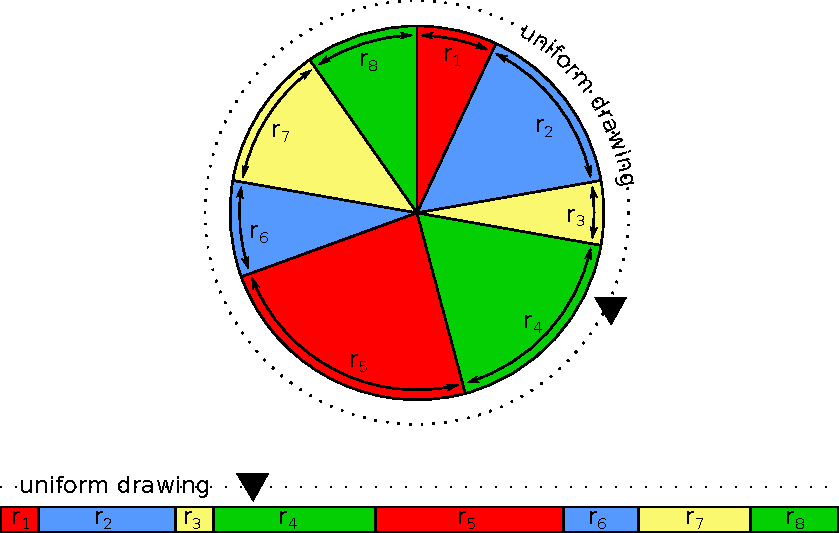
\includegraphics[width=\textwidth]{biased_wheel}
    \end{minipage}
    \begin{minipage}{0.5\textwidth}
      \includegraphics[width=\textwidth]{ratevector_container}
      \includegraphics[width=\textwidth]{ratevector_drawing}
      \includegraphics[width=\textwidth]{ratevector_update}
    \end{minipage}
  \end{minipage}
  \caption{(Left) Illustration of drawing along a biased wheel and its equivalent representation as a segment. (Right) Container and algorithms used to maintain the structure.}
  \label{fig:biased_wheel}
\end {figure}

Generally the wheel is seen as a segment subdivided into $N$ subsegments of length $r_1$, ..., $r_N$. A value $u$ is drawn on this $[0, \sum r_i)$ segment. We proceed iteratively to find to which subsegment $u$ belongs. If $u < r_1$, it belongs to subsegment 1. If $r_1 \leq u < r_1+r_2$, it belongs to subsegment 2, etc.

\subsubsection {Sketch of algorithm and complexity} 

\begin{figure}[!h]
  \begin{minipage}{0.5\textwidth}
    \includegraphics[width=\textwidth]{ratevector_drawing}
  \end{minipage}
  \begin{minipage}{0.5\textwidth}
    \begin{algorithm}[H]
      \KwData{Array r of size N, R = sum (r).}
      \KwResult{Index drawn according to multinomial drawing.}
      u = uniform ([0, R))\;
        index = 1\;
        cum\_sum = r[1]\;
        \While{u $\geq$ cum\_sum}{
          index = index + 1\;
          cum\_sum = cum\_sum + r [index]\;
        }
        \KwRet{index}
    \end{algorithm}
  \end{minipage}
  \caption{Direct drawing method}
  \label{fig:direct_drawing}
\end {figure}

Worst case of the drawing~\reffigp{fig:direct_drawing} occurs when $u$ is in the last subsegment, so the loop has to be iterated $N$ times, yielding $O(N)$ complexity.

\subsection {Next reaction method}

The next reaction method is based on the direct method. It is used in systems where it is known that propensities are not uniform. The point is to accelerate the direct method by sorting (at least rougly) propensities within the vector. This does not change drawing statistics but accelerates finding where a drawing is located on the wheel. For example, say a propensity takes up 50\% of total propensity and is located at the beginning of the vector. Then each random drawing $u < 0.5\sum r_i$ will be instantly found to fall into the first sector of the biased wheel. In a non-sorted vector, we would have to loop through several small sectors before finding the big one.

Because the next reaction method is only a twist of the direct method, we do not go into furter details now. We will also omit it in complexity analysis, as it has the same worst-case complexity as the direct method. We will only reference it again in the Experiment section.

\subsection {Binary tree}

\subsubsection {Principle}

In this approach, we organize propensities inside a tree. Propensities are placed in the leaves of the tree. Nodes are then assembled iteratively 2 by 2 to compute the sum of all propensities~\reffigp {fig:binary_tree}.

\begin{figure}[!h]
  \centering
  \begin{minipage}{0.8\textwidth}
    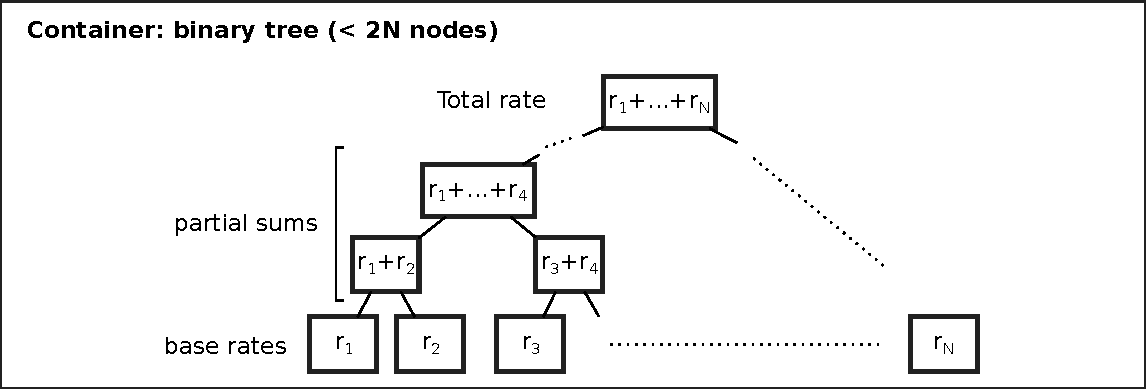
\includegraphics[width=\textwidth]{ratetree_container}
    \includegraphics[width=0.5\textwidth]{ratetree_drawing}
    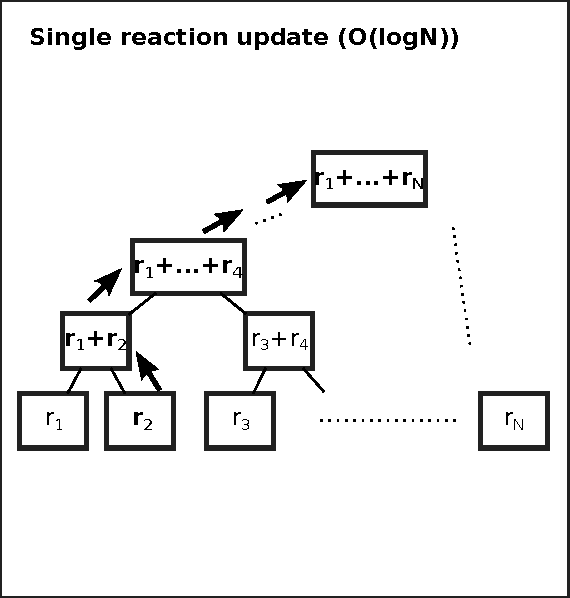
\includegraphics[width=0.5\textwidth]{ratetree_update}
  \end{minipage}
  \caption {Binary tree containing propensities. Propensity values are found at the leaves of the tree. Intermediate nodes represent partial sums of nodes below, root holds the sum of all propensities.}
  \label {fig:binary_tree}
\end {figure}

The idea is that with the structure \emph{in place}, finding the index that has been drawn is quicker. Similarly to the standard drawing, a value $u$ is drawn on the $[0, R=\sum r_i)$ segment. We start from the root node and need to find on which side of the tree $u$ lies. The two children nodes summarize how much weight there is on each side of the tree, say $w_\textrm{left}$ and $w_\textrm{right}$ respectively. If $u < w_\textrm{left}$, we descend to the left child node and proceed the same way until we reach a leaf. If $u \geq w_\textrm{left}$, we descend to the right child and we proceed iteratively with $u = u - w_\textrm{left}$.

This procedure is actually very similar to the biased wheel method, except we perform some kind of progressive zooming in on the subsegments delimited by the propensity values~\reffigp {fig:binary_tree}.

\subsubsection {Sketch of algorithm and complexity} 
\begin{figure}[!h]
  \begin{minipage}{0.5\textwidth}
    \includegraphics[width=\textwidth]{ratetree_drawing}
  \end{minipage}
  \begin{minipage}{0.5\textwidth}
    \begin{algorithm}[H]
      \SetAlgoLined
      \KwData{Binary tree with propensities at its leaves.}
      \KwResult{Index drawn according to multinomial drawing.}
      u = uniform ([0, tree.root.value))\;
        node = tree.root\;
        \While{node is not a leaf}
              {
                \eIf {u $<$ node.left\_child.value}{
                  node = node.left\_child\;
                }{
                  node = node.right\_child\;
                  u = u - node.left\_child.value\;
                }
              }
              \KwRet{node.index}
    \end{algorithm}
  \end{minipage}
  \caption{Binary tree: drawing method.}
  \label{fig:tree_drawing}
\end{figure}

Complexity for performing the drawing~\reffigp{fig:tree_drawing} is given by the depth of the tree, $\lceil\log_2 N\rceil$, which is $O(\log N)$.

\begin{figure}[!h]
  \begin{minipage}{0.5\textwidth}
    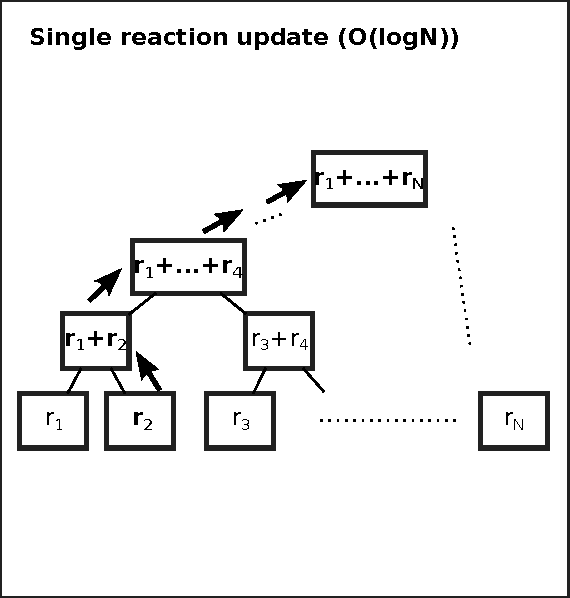
\includegraphics[width=\textwidth]{ratetree_update}
  \end{minipage}
  \begin{minipage}{0.5\textwidth}
    \begin{algorithm}[H]
      \SetAlgoLined
      \KwData{Binary tree with propensities at its leaves. Index i\_update of propensity to update, new propensity value p\_update.}
      \KwResult{Updated binary tree.}
      node = tree.leaf [i\_update]\;
      node.value = p\_update\;
      \While{node is not root}
            {
              node = node.parent\;
              node.value = node.left\_child.value + node.right\_child.value\;
            }
    \end{algorithm}
  \end{minipage}
  \caption{Binary tree: update method.}
  \label{fig:tree_update}
\end{figure}

Complexity for updating the tree~\reffigp{fig:tree_update} is also given by depth of the tree, $O(\log N)$. Note that we need not update every node in the tree, only the parents of the updated leaf up to the root node.


\subsection {Hybrid method}

\subsubsection {Principle}

In this approach, we organize propensities into groups and use a different drawing method: \emph{rejection-base drawing}. This approach has been presented in~\citet{slepoy_constant-time_2008}.

\paragraph{Rejection-based drawing} The aim is to perform a multinomial drawing, similar to what is done by a biased wheel or a binary tree. The problem with the latter methods is that we need to iterate through some structure before finding the right value. With rejection-based drawing, we attempt to \emph{jump} to the right solution. Let $\{r_i\}$ be the propensities of the $N$ reactions in the system and $R = \sum_{1 \leq i \leq N} r_i$.
\begin{enumerate}
\item We choose a value $r_M$ such that $\forall i, r_M \geq r_i$.
\item Until a good candidate is found.
  \begin{enumerate}
  \item We draw a random number $i$ between 1 and $N$ (with replacement).
  \item We draw a random number $u$ on the $[0, r_M]$ segment. If $u > r_i$, we reject $i$, else we keep it.
  \end{enumerate}
\end{enumerate}

A careful proof shows that the probability of drawing index $i$ is equal to $r_i / R$~\citep{serebrinsky_physical_2011}. Note that the choice of $r_M$ is critical for the efficiency of the method~\reffigp[A]{fig:rejection_based_drawing}. Formally, the probability to accept a candidate is $\sum_i\prob{\textrm{draw }i}$ $\prob{\textrm{accept }i} = \sum_i1/N \times r_i/r_M = R/(Nr_M)$. If applied naively, the number of candidates to loop through is a geometric law with parameter $R/(Nr_M)$. The expected number of candidates is thus $Nr_M/R$. For a uniform distribution, this value can be 1, but in general, it yields bad results~\reffigp[B]{fig:rejection_based_drawing}.

\begin{figure}[!h]
  \centering
  \begin{minipage}{0.59\textwidth}
    \textbf{A} \\
    \includegraphics[width=\textwidth]{rejection_principle}
  \end{minipage}
  \begin{minipage}{0.39\textwidth}
    \textbf{B} \\
    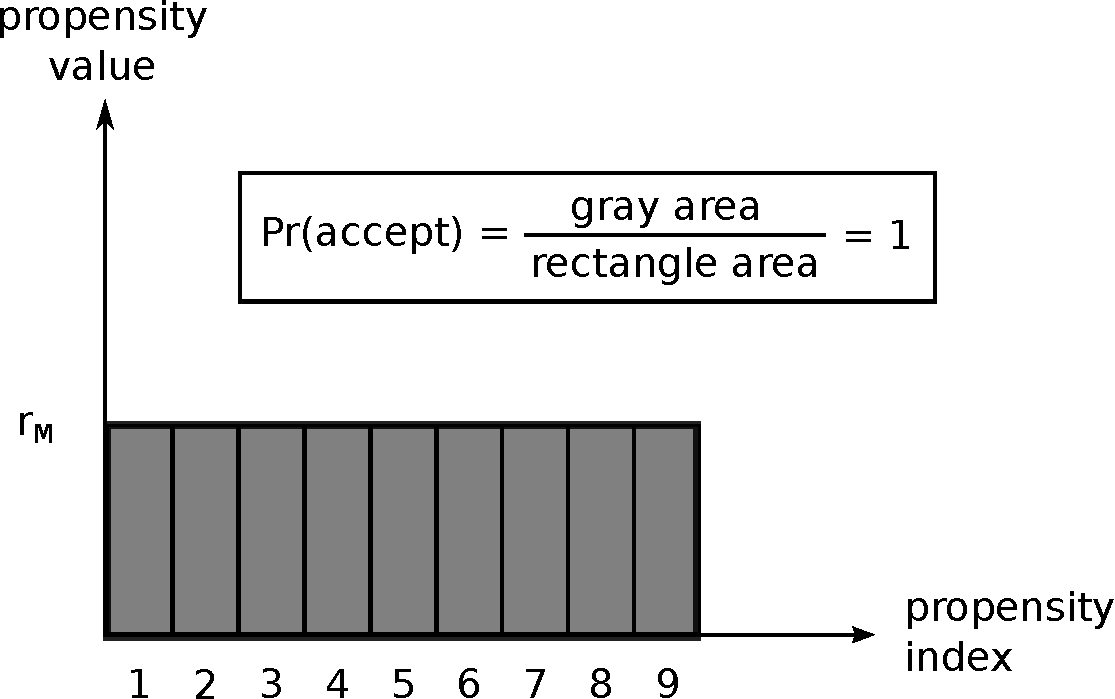
\includegraphics[width=\textwidth]{rejection_uniform}
    \includegraphics[width=\textwidth]{rejection_bad}
  \end{minipage}
  \begin{minipage}{0.6\textwidth}
    \textbf{C}\\
    \includegraphics[width=\textwidth]{rejection_groups}  
  \end{minipage}
  \caption{Rejection based drawing (adapted from \citet{slepoy_constant-time_2008}). (A) Geometric illustration of rejection principle. Drawing occurs in a 2D space, with propensities aligned along the $x$ axis and their value given by gray bars along the $y$ axis. A drawing is accepted if it falls into the gray domain. Note that the probability to draw a propensity is proportional to its value, as an accepted drawing will be distributed uniformly across the gray domain. (B) Examples displaying efficiency of the technique (maximal for uniform propensities, minimal when some are very high and most are very low). (C) Sorting propensities into groups whose limits are powers of 2 ensures a minimal 1/2 acceptation probability \emph{within a given group}.}
  \label{fig:rejection_based_drawing}
\end {figure}

 \paragraph{Group method} The idea behind the algorithm is to improve the acceptation probability by placing propensities in \emph{groups}:
\begin{enumerate}
\item We draw a group index by using a classical method (biased wheel or binary tree).
\item We draw a propensity inside the group by using the rejection-based method.
\end{enumerate}

\citet{slepoy_constant-time_2008} propose placing propensities into binary groups. They choose a base rate $b$. Groups are of the form $(0, b]$, $(b, 2b]$, $(2b, 4b]$, \textit{etc.} $(0,b]$ contains all propensities between 0 and $b$, and so on. When applying the rejection method to any of these groups (except $(0, b]$), the acceptation probability is $\geq 1/2$~\reffigp[C]{fig:rejection_based_drawing}. Note that the number of groups $K$ does not generally depend on $N$, it only depends on the highest propensity value. In general, it remains relatively small.

Suppose the structure is already in place, \textit{i.e.} propensities are placed in the right group and the total propensity for each group is known. Step 1 is at most $O(K)$, which is independent of $N$. Step 2 requires less than 2 candidates on average, so it is $O(1)$. This results in $O(1)$ globally, making it significantly more efficient than the two previous methods. However, we will see that its implementation is also trickier in order to preserve this theoretical complexity.

\begin{figure}[!h]
  \centering
  \includegraphics[width=0.8\textwidth]{hybrid_container}
  \includegraphics[width=0.8\textwidth]{hybrid_drawing}
  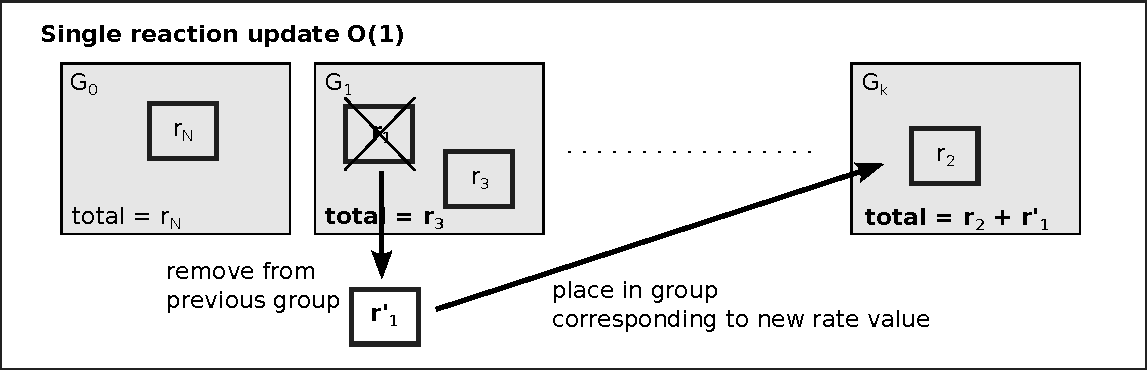
\includegraphics[width=0.8\textwidth]{hybrid_update}
  \caption {Hybrid method using group structure and rejection algorithm.}
  \label {fig:hybrid_method}
\end {figure}

\subsubsection {Sketch of algorithm and complexity} 

\begin{figure}[!h]
  \centering
  \begin{minipage}{\textwidth}
    \centering
    \includegraphics[width=0.8\textwidth]{hybrid_drawing}
    \begin{algorithm}[H]
      \SetAlgoLined
      \KwData{$K+1$ groups, group k containing propensities whose value falls in the interval $(0,b]$ if k=0, $(2^{k-1}b, 2^kb]$ if k $>$ 0. Propensities are stored as a couple containing their value and original index.}
      \KwResult{Index drawn according to multinomial drawing.}
      \tcp {drawing using a direct method like binary tree or biased wheel}
      group = groups [multinomial (group[0].total\_propensity, ..., 
        group[K].total\_propensity)]\;
      \Repeat{candidate.value $>$ uniform (0, group.max\_propensity)}{
        candidate = group.propensities [uniform (1, group.number\_propensities)]\;
      }
      \KwRet{candidate.index}
    \end{algorithm}
  \end{minipage}
  \caption{Hybrid method: drawing method.}
  \label{fig:hybrid_drawing}
\end{figure}

Because of the group structure, the loop in \reffigt{fig:hybrid_drawing} is $O(1)$ (see above). The first multinomial drawing is at most $O(K)$, so the complexity is globally $O(K)$. Because $K$, the number of groups, does not naturally scale with $N$, the number of reactions, the complexity is overall $O(1)$, as $N$ is the real variable of interest here.


\begin{figure}[!h]
  \centering
  \begin{minipage}{\textwidth}
    \centering
    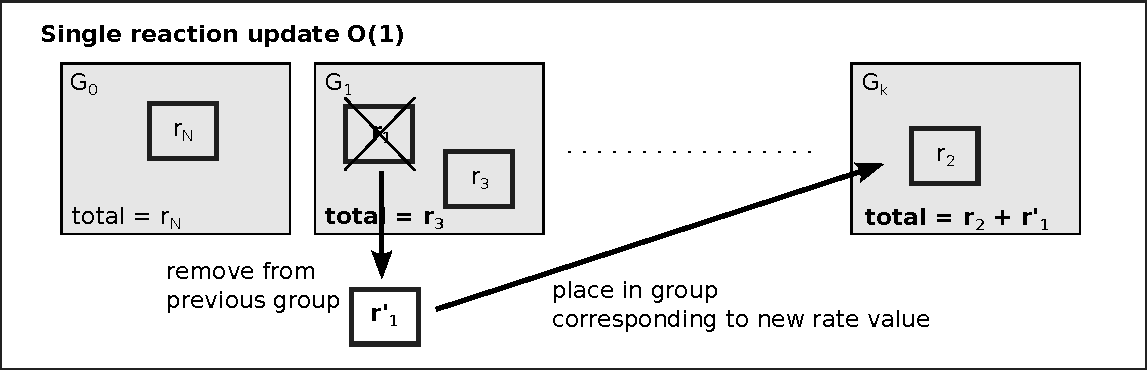
\includegraphics[width=0.8\textwidth]{hybrid_update}
    \begin{algorithm}[H]
      \SetAlgoLined
      \KwData{$K+1$ groups, group k containing propensities whose value falls in the interval $(0,b]$ if k=0, $(2^{k-1}b, 2^kb]$ if k $>$ 0. Propensities are stored as a couple containing their value and original index. Index i\_update of propensity to update, new propensity value p\_update.}
  \KwResult{Updated group structure.}
  \Fn {group\_index (propensity)}{
    \eIf{propensity $\geq$ b}{
      \KwRet{$\lceil \log_2 (\textrm{reaction.propensity} / b) \rceil$}
    }{
      \KwRet {0}
    }
  }
  propensity = propensity corresponding to index i\_update\;
  previous\_group = groups [group\_index (propensity.value)]\;
  Remove propensity from previous\_group and update group's total propensity\;
  new\_group = groups [group\_index (p\_update)]\;
  propensity.value = p\_update\;
  Add propensity to new\_group and update group's total propensity\;
    \end{algorithm}
  \end{minipage}
  \caption{Hybrid method: update method.}
  \label{fig:hybrid_update}
\end{figure}

At first sight, updating the group structure is also $O(1)$~\reffigp{fig:hybrid_update}. However, the parts about removing or inserting a reaction into a group must be carefully implemented in order to achieve that result.

\subsection {Summary}

\reftabt{tab:selection_summary} summarizes the worst case complexity of four methods presented. Note that the update complexity was derived in the case where onle one propensity needed to be updated. To obtain the overall complexity, we need to take into account the number of reactions $U$ whose propensity needs to be updated. A naive analysis indicates that the binary tree could be less efficient than the direct method depending on $U$ and $N$~\reftabp{tab:selection_summary}. In the next section, we will analyze how $U$ can influence the efficiency of each method.

\begin{table}[!h]
  \centering
  \begin{tabular}{|l|c|c|c|}
    \hline
    Method & Drawing Complexity & Update Complexity & Total Complexity\\
           &                    & (one propensity) & \\
    \hline
    Direct Method & $O(N)$ & $O(1)$ & $O(N)$?\\
    Binary Tree & $O(\log N)$ & $O(\log N)$ & $O(U\log N)$?\\
    Hybrid Method & $O(1)$ & $O(1)$ & $O(U)$?\\
    \hline
  \end{tabular}
  \caption{Comparison of worst-case complexities of methods presented here. $N$ is the number of reactions in the system, $U \leq N$ the number of reactions whose propensity needs to be updated. The last column is a projection based on the first two columns, real total complexities are given in the next section.}
  \label{tab:selection_summary}
\end{table}	

\section {Propensity updating}
\label{sec:reaction_update}

In \refsect{sec:reaction_selection}, we have introduced methods to perform a multinomial drawing among $N$ propensity values. We have seen that special structures can improve the drawing time but there is an additional cost to update those structures when a propensity value changes. Here we will study how this additional cost evolves when $U$ propensities need to be changed from one drawing to the next drawing.

\subsection {Naive method: why not update everything?}

We begin with the simple case where $U = N$.

\paragraph{Direct Method} In the direct method, we need to compute the total propensity of the system, so we need to loop through all propensities at least once. In this sense, the overall update complexity is $O(N)$ and the total comlexity (including drawing) is equally $O(N)$.

\paragraph{Binary Tree} We need to update all leaves of the tree. Naively, this would lead to a $O(N\log N)$ overall update complexity. However, this assumes that each time a leaf value is updated, we update all the intermediate nodes up to the root. In practice, it is possible to differ update of intermediate nodes and just mark them as outdated. We only udpate them once all their children have been treated, so that every node is udpated at most once. In the case where all leaves are updated, every node in the tree is updated exactly once. The complexity is thus given by the number of nodes in the tree, approximately $2N$, yielding $O(N)$ overall update complexity. The total complexity is then $O(\log N + N) = O(N)$.

\paragraph{Hybrid Method} Here the update algorithm is applied to every propensity, yielding a overall $O(N)$ update complexity. Total complexity is $O(1 + N) = O(N)$.

\paragraph{Summary} As a matter of fact, when propensities are updated naively, the benefit of using sophisticated structures is (asymptotically) lost~\reftabp{tab:naive_update}.
\begin{table}[!h]
  \centering
  \begin{tabular}{|l|c|c|c|}
    \hline
    Method & Drawing Complexity & Update Complexity & Total Complexity\\
    \hline
    Direct Method & $O(N)$ & $O(N)$ & $O(N)$\\
    Binary Tree & $O(\log N)$ & $O(N)$ & $O(N)$\\
    Hybrid Method & $O(1)$ & $O(N)$ & $O(N)$\\
    \hline
  \end{tabular}
  \caption{Worst-case complexities for $U=N$.}
  \label{tab:naive_update}
\end{table}	

It is absolutely necessary to keep $U$ as small as possible. Formally, we need to determine a subset of propensities that includes all propensities that might have changed. In that case, specific drawing structures start to be interesting~\reftabp{tab:general_update}. Roughly speaking, the binary tree is better than the direct method as soon as $U < N / \log N$ and the hybrid method outcompetes the two other methods for $U < N$.

This trend is even stronger in a system where the number of propensities to update does not depend on $N$~\reftabp{tab:ideal_update}. In this case, the direct method is linear, the binary tree logarithmic and the hybrid method constant time, yielding huge improvements when switching from one method to the next one. 

Keep in mind that those are asymptotic trends, that will become clearer for large $N$. If the system is small, other terms may prevail that depend on implementation details. We will see what large means in \refsect{sec:experiments}.

But first, we are going to focus on $U$. How does it scale with $N$ in a specific system? And how can we keep it as small as possible?

\begin{table}[!h]
  \centering
  \begin{tabular}{|l|c|c|c|}
    \hline
    Method & Drawing Complexity & Update Complexity & Total Complexity\\
    \hline
    Direct Method & $O(N)$ & $O(U)$ & $O(N)$\\
    Binary Tree & $O(\log N)$ & $O(\min\{U\log N,N\})$ 
    & $O(\min\{U\log N,N\})$\\
    Hybrid Method & $O(1)$ & $O(U)$ & $O(U)$\\
    \hline
  \end{tabular}
  \caption{Worst-case complexities for a general $U \leq N$.}
  \label{tab:general_update}
\end{table}	

\begin{table}[!h]
  \centering
  \begin{tabular}{|l|c|c|c|}
    \hline
    Method & Drawing Complexity & Update Complexity & Total Complexity\\
    \hline
    Direct Method & $O(N)$ & $O(1)$ & $O(N)$\\
    Binary Tree & $O(\log N)$ & $O(\log N)$ & $O(\log N)$\\
    Hybrid Method & $O(1)$ & $O(1)$ & $O(1)$\\
    \hline
  \end{tabular}
  \caption{Worst-case complexities for the ideal case $U=O(1)$ (number of propensities to update does not scale with the number of reactions $N$ in the system).}
  \label{tab:ideal_update}
\end{table}	

\subsection{Using graphs to update propensities}

The most standard way to study how reactions influence each other is to draw a graph that tracks the dependencies between reactions. A first version can be drawn using a \emph{bipartite graph} with reactions on one side and reactants on the other one. When can draw two sets of vertices~\reffigp{fig:reactant_reaction_graph}.
\begin{itemize}
  \item If the reaction modifies the concentration of a reactant, a directed vertex is drawn from the reaction to the reactant.
  \item If the concentration of a reactant is used to compute the propensity of a reaction, a directed vertex is drawn that goes from the reactant to the reaction.
\end{itemize}

\begin{figure}[!h]
  \centering
  \begin{minipage}{0.39\textwidth}
    \[
    \begin{array}{l}
      R_1:\reactionIrr{A}{C+D}{}{} \\
      R_2:\reactionRev{B+C}{E}{}{} \\
      R_3:\reactionIrr{B+E}{2A}{}{} \\
      R_4:\reactionIrr{D+A}{B+A}{}{}
    \end{array}
    \]
  \end{minipage}
  \begin{minipage}{0.59\textwidth}
    \includegraphics[width=\textwidth]{graphs}
  \end{minipage}
  \caption{(Left) Sample reaction system. (Right) Corresponding bipartite graph displaying interactions between reactions and reactants. The reaction nodes were duplicated for readability.}
  \label{fig:reactant_reaction_graph}
\end{figure}

\subsubsection{Reactant to reaction graph}

The first algorithm we propose only takes advantage of the set of vertices that goes from reactants to reactions. Here is the sketch of the algorithm:
\begin{itemize}
  \item We set up an \emph{observer pattern} to track changes in concentrations. Schematically, every time the concentration of a reactant changes, the reactant sends an update that will \emph{invalidate} the propensities in which it is involved (as pointed by the vertices on the graph).
  \item We initialize the system by computing all propensities.
  \item Until some target is reached:
    \begin{itemize}
      \item A random reaction is performed. Concentration of some reactant changes. Updates are sent and some propensities are invalidated.
      \item We recompute the propensities that were invalidated.
    \end{itemize}
\end{itemize}

\subsubsection{Reaction to reaction graph}

In the second algorithm, we collapse the bipartite graph shown above into a graph that only contains reactions. The collapsing process is rather intuitive if we use the directed vertices defined above. Take two reactions $A$ and $B$. There is a vertex $A \rightarrow B$ if there is some reactant $R$ such that $A \rightarrow R$ and $R \rightarrow B$ in the bipartite graph. Put into words: when reaction $A$ occurs, it changes the concentration of a reactant $R$ used to compute the propensity of $B$~\reffigp{fig:reaction_reaction_graph}. 

\begin{figure}[!ht]
  \centering
  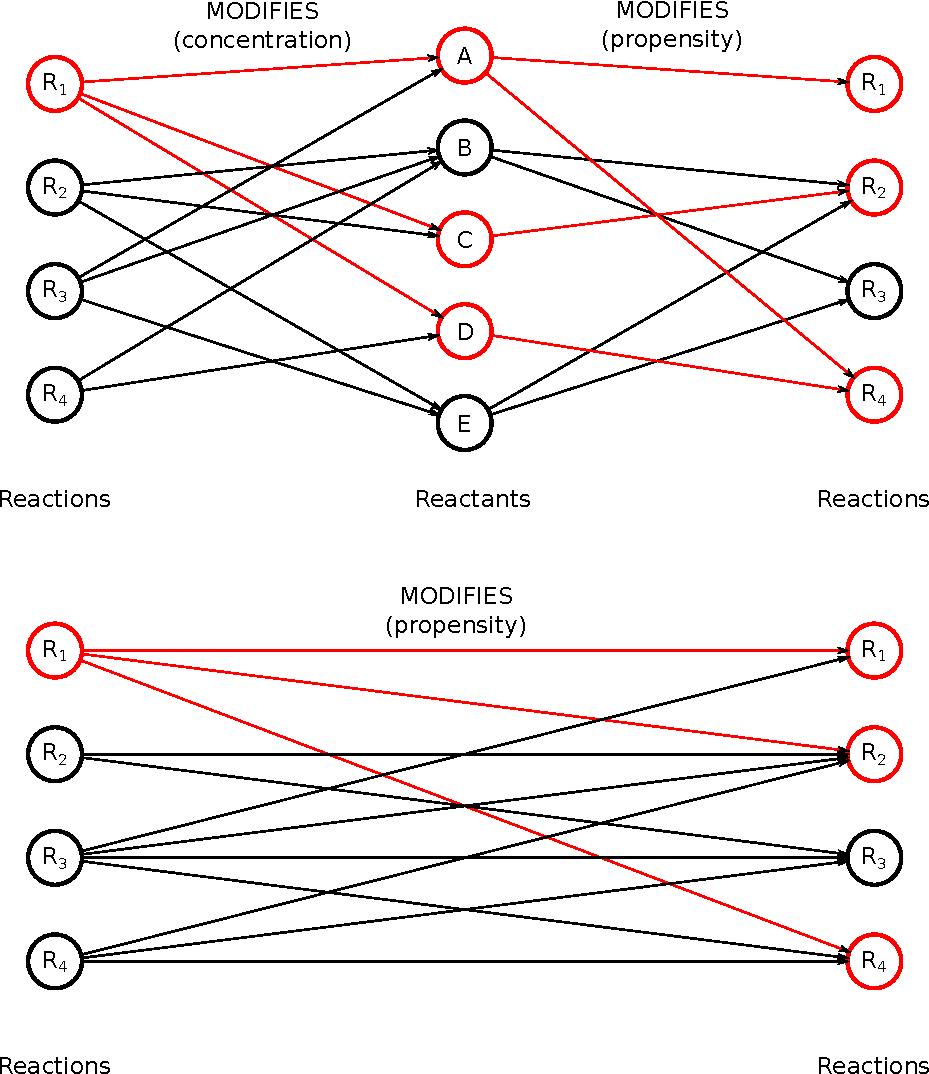
\includegraphics[width=0.6\textwidth]{graph_reaction_reaction}
  \caption{Collapsing bipartite graph into a pure reaction graph. (Top) Example of collapsing for reaction $R_1$. All paths leading to a potential propensity change in other reactions are displayed in red. (Bottom) Reaction to reaction graph. In red are the vertices that correspond to the paths displayed in red in the bipartite graph. Reaction nodes were duplicated for readability, the graph could also be represented with only one node for each reaction.}
  \label{fig:reaction_reaction_graph}
\end{figure}

Here is a sketch of the algorithm:
\begin{itemize}
  \item We create the reaction graph: for each reaction we store the list of propensities to update when it occurs.
  \item We initialize the system by computing all propensities.
  \item Until some target is reached:
    \begin{itemize}
      \item A random reaction is performed.
      \item We recompute the propensities according to the reaction graph.
    \end{itemize}
\end{itemize}

\subsubsection{Pros and cons}

\paragraph{Preliminary analysis} The main difference between the algorithms is that the reactant to reaction algorithm uses an observer pattern. This pattern it slightly more complicated to implement than the reaction graph. Moreover, in closed systems of chemical reactions, the reaction graph approach is more efficient. We can perform a very simple cost analysis for the update occurring after one reaction has been performed.

\begin{itemize}
  \item Rectant to reaction graph: for every reactant involved in the reaction, an update is sent that invalidates a subset of propensities. The subsets invalidated by the reactants might overlap, resulting in invalidating the same propensity several times. Note that invalidating does not mean recomputing the propensity, it is only recomputed after the whole invalidation process if it has been tagged by at least one reactant.
  \item Reaction to reaction graph: when the reaction occurs, we have direct access to the subset of propensities to recompute.
\end{itemize}

We see that there are additional costs in the reactant to reaction method because of the update sending and possible overlaps that are eliminated when the reactant to reaction graph is collapsed into the simpler reaction graph. Depending on the system, these additional costs may not be negligible, even though they should remain fairly low.

\paragraph{System with external constraints} If something else than a reaction might change the concentration of a reactant, propensities will be updated correctly only when using the reactant to reaction algorithm. When using the reaction graph, such interactions are not visible and it may be necessary to update all propensities every time such an event occurs.

This flexibility problem can be overcome without an observer pattern by storing both the reaction graph \emph{and} the bipartite graph to use the reactant to reaction graph when needed. However, the solver still needs to be notified every time the concentration of a reactant changes due to external reasons. There is a danger that this notification might be omitted by the programmer, while an observer pattern guarantees that the solver will be aware of such changes.

\paragraph{System containing agregated reactions} In more complex systems that do not only include chemical reactions, it is possible to include reactions that have multiple outcomes. We developed a simulator that includes a \texttt{Loading} reaction. A typical example is a RNA polymerase building a RNA by matching either an ATP, a CTP, a GTP or a UTP depending on the DNA base it is reading. The base is read dynamically during simulation, so we do no know in advance which NTP pool is going to be impacted by the reaction. 

In this case, when collapsing the reactant to reaction graph, we would need to consider all possible outcomes. We would end up updating all propensities involving ATP, CTP, GTP and UTP, even though only one NTP was really affected. The reactant to reaction graph is more efficient in this case, as updates are only sent for the NTP effectively used, leading to fewer propensity computations.

\paragraph{System containing complex dependencies between reactions} An even trickier issue are hidden dependencies between reaction. Let us quote an example from our simulator again. It contains a \texttt{SequenceBinding} reaction, where a molecule can bind on a binding site, \textit{e.g.} a transcription factor binding on DNA at a specific site. The propensity depends on the availability of the transcription factor but also the availability of the binding site. Suppose a DNA polymerase happens to hide the binding site, how can we make sure the binding propensity reflects the unavailability of the binding site?

With a reaction to reaction graph, it is difficult to account for that situation in a comfortable way. We might be tempted to introduce special interactions between instances of reactions (translocation of a polymerase \emph{may} change binding propensity). In our opinion, this would lead to bad software. Why? Let us compare with the reactant to reaction approach. We can declare a binding site to be a reactant that gets notified every time its availability changed. This is enough to ensure that all propensities will be updated properly. Implementation is simple and transparent. Everything is based on a single abstraction (reactant concentrations determine propensities): no painful special cases.

\begin{footnotesize}
  Remark: There are ways to handle hidden dependency problems without using the observer pattern. We may choose to make propensity of \texttt{SequenceBinding} reactions independent of site availability by using a rejection method. Propensity is computed from number of sites, available or not. When reaction is performed by solver, a binding is \emph{attempted} on a random site. If site is free: reaction is effectively performed, if it is occupied: reaction is \emph{ignored}. This is statistically equivalent to the observer system described in the previous graph. However, note that this does not really solve the problem, as propensity still needs to be updated properly when the number of sites changes. In our simulator, number of sites can be a non-trivial property (\textit{i.e.} it is not the result of any particular reaction, but the outcome of a process -- replication -- involving a lot of different reactions). Also note that rejecting a reaction is pretty costly, so this turnaround might be more expensive than using an observer pattern if binding sites tend to be occupied frequently.
\end{footnotesize}

\subsubsection{Conclusion}

In simple systems, the reaction graph is both superior in speed and easier to implement. In more complex systems, the reactant to reaction graph proves to be significantly more flexible and possibly more efficient. We implemented both algorithms in our simulator. At the beginning, when using simple reaction systems, the reaction graph algorithm was slightly superior. When simulating more complex systems, the reaction graph proved to be nearly impossible to maintain. Even though it may be slightly more costly in simple cases, the reactant to reaction graph provides a better abstraction when extending towards more complex systems. Implementation remains easy and \emph{safe}: propensities are updated the way they should. This became harder and harder to achieve using the reaction to reaction approach, so we ended up abandonning it in our simulator.


\subsection {Experiments}
\label{sec:experiments}

\section {Perspectives}

\paragraph{Selection reaction: tau-leaping}

\paragraph{Propensity updationg: factorizing reactions}

\paragraph {Implementation: parallel computing}


\appendix

\section{Implementation details}
\label{sec:implementation_details}

Implementation details fall into two categories. Optimization concerns ensure that implementations yield the claimed theoretical complexity. Numerical concerns address rounding problems that occur quite frequently in real-word situations.

When optimization is addressed, structures and algorithms are proposed that yield the asymptotic complexities presented in this document. Only rarely do we insist on optimizations that will only improve the multiplicative or additive constants of the algorithms. The reader is free to use its own adapted/further optimized structures.

Numerical issues are dangerous as algorithms ignoring them may lead to plausible, yet statistically flawed, results. They \emph{must} be addressed at all costs. We propose simple ways to treat them. We do not doubt that more rigorous treatments exist.

\subsection{Numerical concern: updating total propensity on the fly}
\label{ssec:total_numerical}
We start with numerical issues, as all methods are impacted by rounding problems. For illustrative purposes, we focus on the computation of the total of a set of real values.

\paragraph{Context} Suppose we have a vector $v$ of $n$ real values. The task is to maintain the total value $T := \sum_{1\leq i\leq n}v[i]$. Computing $T$ anew every time a value changes is too expensive. Suppose we want to set $v[i]$ to a new value $new\_v\_i$. Theoretically, the new value of $T$ will be $T - v[i] + new\_v\_i$. 

\paragraph{Numerical issue: absorption} On a computer, such operations will \emph{always} lead to rounding problems. In other words, we must be aware that $T$ will always be different from the real total. Question is: how different? Here we need to get a little technical and talk about the problem of \emph{absorption}. Rougly speaking, a 64 bit \texttt{double} has a precision of 15 to 17 digits, the rest can be ignored. Take some number $a$. The next \texttt{double} a machine can represent is roughly $a + 10^{-15}a$. If we add $b$ such that $b < 10^{-16}a$, rounding leads to $a+b=a$: $a$ \emph{absorbs} $b$. Now imagine $b \simeq 10^{-n}a$ where $1 \leq n \leq 15$. $b$ is no longer absorbed by $a$, but its original precision will be lost in operations such as $b+a-a$. The first operation treated is $b+a$, where only $\simeq 16-n$ digits of $b$ that fall in the meaningful region of $a$ are really kept~\reffigp{fig:absorption}. When $a$ is removed, only these digits are restored: $b$ is left with only $16-n$ meaningful digits. To track absorption, we need to know how the \emph{largest} number treated in our operations compares to the current total. Let $M$ be that number and $T$ the total introduced in the context paragraph. The number of meaningful digits of $T$ is $\simeq 16 - \lceil\log_{10}M - \log_{10}T\rceil$.

\begin{figure}[!h]
  \centering
  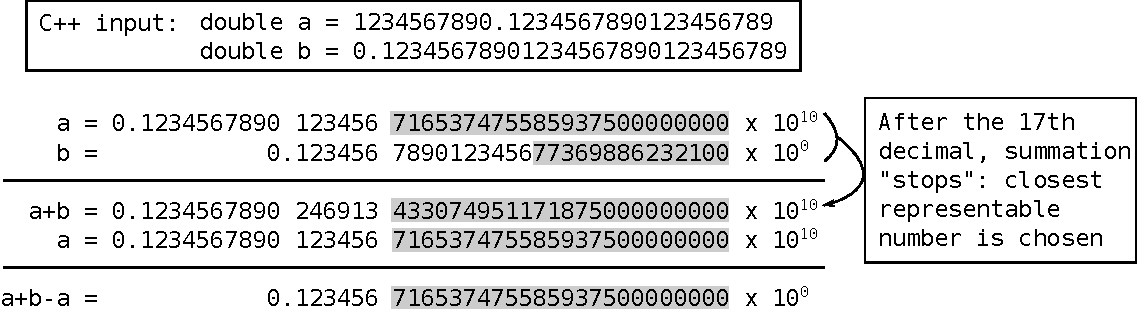
\includegraphics[width=\textwidth]{absorption}
  \caption{Illustration of a rounding problem due to absorption. Gray areas show the decimals the computer has no real control of. They are chosen according to closest representation available. When summing terms, the sum can only be exact up to 17 decimals at most, so a part of the decimals of the smaller term of the sum are ignored and cannot be recovered. }
  \label{fig:absorption}
\end{figure}

\paragraph{Solutions} One possible solution is to switch to higher precision. 128 bit \texttt{quadruple} offer 33 to 36 meaningful digits, spanning a larger range of magnitudes. But even with larger precision, it may be necessary to track the current precision of $T$. This can be achieved by recording the largest number $M$ used to compute $T$ and use $d = 16 - \lceil\log_{10}M - \log_{10}T\rceil$ (replace 16 with 34 for \texttt{quadruple}) as a proxy for the number of meaningful digits. Because of rounding problems affecting meaningful digits, this is rather an optimistic estimate. When $d$ falls below a predefined limit (somewhere between 5 and 10), $T$ has to be recomputed from scratch. This operation can also be dangerous in various ways (if $v$ has a lot of small values and a large value, compensation of large numbers that have opposite sign). In practice, these dangers do not naturally arise in our case, but they can be treated by sorting the numbers by magnitude and carefully considering the order in which they are added up.

\subsection{Direct Method}
The only concern with this method is to update the total propensity properly~\refsecp{ssec:total_numerical}.

\subsection{Binary Tree}

\subsubsection{Updating intermediate nodes at most once}
This optimization is pretty straightforward. The tree is updated starting from the highest depth. We suppose the tree is built so that all leaves are at the same depth. We use an update queue that initially contains all nodes whose propensities are outdated. 

We follow this simple rule: every time a node is updated, its parent is added to the update queue. Each node holds an \texttt{outdated} flag. If a node is marked \texttt{outdated}, we know it is already in the queue and we do not add it a second time. The flag is removed when the node is updated. 

By applying this procedure, nodes are added layer by layer. As mentionned above, we start with leaves at the highest depth. As we progress through leaves, there parents are added at their succession and so on, until root is finally reached. By using the flag system, each node is queued and updated at most once.

Note that the update queue will at most contain all nodes of the tree, \textit{i.e.} $\simeq 2N$ nodes. To avoid memory reallocation, it can (should) be represented by an array of size $2N$ and two pointers to the start and end of the queue. 

This procedure can be adapted if the leaves are not all at the same depth.

\subsubsection{Numerical concern: rounding problems}

\subsection{Hybrid Method}

\subsubsection{Numerical concerns}

\subsubsection{Efficient inserting/removal in groups}

\subsubsection{Choice of base rate}



\bibliographystyle{myplainnat}
\bibliography{cati}

\end{document}
% ----------------------------------------------------------------
